\documentclass[border=15pt, multi, tikz]{standalone}
\usepackage{import}
\usepackage{etoolbox}
\usepackage{graphicx}
\usepackage{svg}
\usepackage{colortbl}

\usetikzlibrary{positioning,matrix,fit}
\usetikzlibrary{3d} %for including external image
\usetikzlibrary{decorations,shapes}
\usetikzlibrary{decorations.shapes}
\usetikzlibrary{decorations.markings}
\usetikzlibrary{decorations.pathreplacing}
\usetikzlibrary{backgrounds}
\usetikzlibrary{calc}
\usetikzlibrary{arrows.meta,arrows}
\graphicspath{{image/}}

\colorlet{blockColor}{blue!80!black}
\colorlet{cellColor}{green!80!black}

\tikzset{%
  % Specifications for style of nodes:
    >={Latex[width=2mm,length=2mm]},
    window/.style = {rectangle, minimum width=6em, minimum height=8em, draw, very thick,anchor=north west},
    slit/.style={rectangle, minimum width=3em, minimum height=8em, draw=orange!60!black, very thick,anchor=north west},
    block/.style={rectangle, minimum width=3em, minimum height=4em, draw=blue!80, very thick,anchor=north west},
    cell/.style={rectangle, minimum width=1.5em, minimum height=2em, draw=green!80, very thick,anchor=north west},
}


\begin{document}
\begin{tikzpicture}[node distance=1em]

\node[window] (slits) at (0,0) {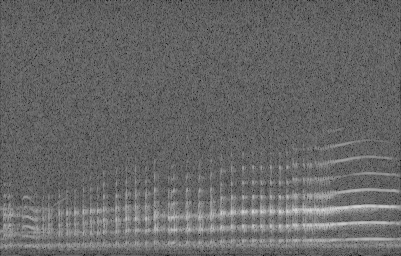
\includegraphics[width=6em,trim=215 0 0 0, clip]{input.png}};
\node[slit, opacity=0.2] at (.4em, -.4em) {};
\node[slit, opacity=0.4] at (1.2em, -.4em) {};
\node[slit] (slit1) at (2em, -.4em) {};
% \node[left = of slit1] {$y$};
% \node[below = 0em of slit1, fill=white] {\textcolor{red}{$x$}};
\node[above=of slit1,draw=orange!60!black] (slit1label) {slit};
\draw[draw=orange!60!black] (slit1) -- (slit1label);

\node[slit, right=of slits, inner sep=0,draw=orange!20!black, xshift=1em] (blocks) {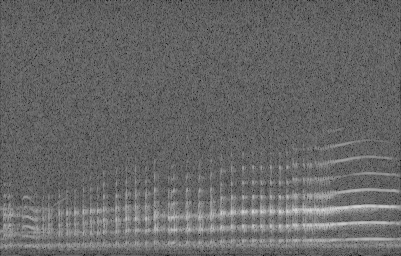
\includegraphics[width=3em,trim=275 0 30 0, clip]{input.png}};
\node[block, opacity=0.4] (block1) at (blocks.north west) {};
\node[block, opacity=0.4] (block3) at (block1.south west) {};
\node[block, yshift=2em] (block2) at (block1.south west) {};
\node[above=of block1, draw=blue!80!black] (block2label) {block};
\node[below = .5em of block3] {$W\times H$ cells};
\draw[draw=blockColor] (block2) -- (block2label);

\node[block, right=of blocks, inner sep=0,draw=orange!20!black, xshift=1em] (cells) {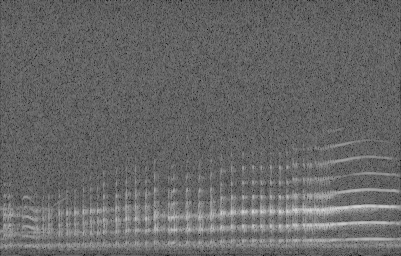
\includegraphics[width=3em,trim=275 60 30 60, clip]{input.png}};
\node[cell, opacity=0.4] (cell1) at (cells.north west) {};
\node[cell, xshift=-1] (cell2) at (cell1.north east) {};
\node[cell, opacity=0.4] (cell3) at (cell1.south west) {};
\node[cell, opacity=0.4] (cell4) at (cell2.south west) {};
\node[below = .5em of cell3,xshift=.75em] {$W\times h$ cells};
\node[above=of cell2,draw=cellColor] (cell2label) {cell};
\draw[draw=cellColor] (cell2) -- (cell2label);

\draw[->,draw=orange!60!black,very thick] (slit1) -- (blocks);
\draw[->,draw=blue!80!black,very thick] (blocks) -- (cells);

\end{tikzpicture}
\end{document}